% GNUPLOT: LaTeX picture with Postscript
\begingroup
  \makeatletter
  \providecommand\color[2][]{%
    \GenericError{(gnuplot) \space\space\space\@spaces}{%
      Package color not loaded in conjunction with
      terminal option `colourtext'%
    }{See the gnuplot documentation for explanation.%
    }{Either use 'blacktext' in gnuplot or load the package
      color.sty in LaTeX.}%
    \renewcommand\color[2][]{}%
  }%
  \providecommand\includegraphics[2][]{%
    \GenericError{(gnuplot) \space\space\space\@spaces}{%
      Package graphicx or graphics not loaded%
    }{See the gnuplot documentation for explanation.%
    }{The gnuplot epslatex terminal needs graphicx.sty or graphics.sty.}%
    \renewcommand\includegraphics[2][]{}%
  }%
  \providecommand\rotatebox[2]{#2}%
  \@ifundefined{ifGPcolor}{%
    \newif\ifGPcolor
    \GPcolortrue
  }{}%
  \@ifundefined{ifGPblacktext}{%
    \newif\ifGPblacktext
    \GPblacktexttrue
  }{}%
  % define a \g@addto@macro without @ in the name:
  \let\gplgaddtomacro\g@addto@macro
  % define empty templates for all commands taking text:
  \gdef\gplbacktext{}%
  \gdef\gplfronttext{}%
  \makeatother
  \ifGPblacktext
    % no textcolor at all
    \def\colorrgb#1{}%
    \def\colorgray#1{}%
  \else
    % gray or color?
    \ifGPcolor
      \def\colorrgb#1{\color[rgb]{#1}}%
      \def\colorgray#1{\color[gray]{#1}}%
      \expandafter\def\csname LTw\endcsname{\color{white}}%
      \expandafter\def\csname LTb\endcsname{\color{black}}%
      \expandafter\def\csname LTa\endcsname{\color{black}}%
      \expandafter\def\csname LT0\endcsname{\color[rgb]{1,0,0}}%
      \expandafter\def\csname LT1\endcsname{\color[rgb]{0,1,0}}%
      \expandafter\def\csname LT2\endcsname{\color[rgb]{0,0,1}}%
      \expandafter\def\csname LT3\endcsname{\color[rgb]{1,0,1}}%
      \expandafter\def\csname LT4\endcsname{\color[rgb]{0,1,1}}%
      \expandafter\def\csname LT5\endcsname{\color[rgb]{1,1,0}}%
      \expandafter\def\csname LT6\endcsname{\color[rgb]{0,0,0}}%
      \expandafter\def\csname LT7\endcsname{\color[rgb]{1,0.3,0}}%
      \expandafter\def\csname LT8\endcsname{\color[rgb]{0.5,0.5,0.5}}%
    \else
      % gray
      \def\colorrgb#1{\color{black}}%
      \def\colorgray#1{\color[gray]{#1}}%
      \expandafter\def\csname LTw\endcsname{\color{white}}%
      \expandafter\def\csname LTb\endcsname{\color{black}}%
      \expandafter\def\csname LTa\endcsname{\color{black}}%
      \expandafter\def\csname LT0\endcsname{\color{black}}%
      \expandafter\def\csname LT1\endcsname{\color{black}}%
      \expandafter\def\csname LT2\endcsname{\color{black}}%
      \expandafter\def\csname LT3\endcsname{\color{black}}%
      \expandafter\def\csname LT4\endcsname{\color{black}}%
      \expandafter\def\csname LT5\endcsname{\color{black}}%
      \expandafter\def\csname LT6\endcsname{\color{black}}%
      \expandafter\def\csname LT7\endcsname{\color{black}}%
      \expandafter\def\csname LT8\endcsname{\color{black}}%
    \fi
  \fi
  \setlength{\unitlength}{0.0500bp}%
  \begin{picture}(7200.00,5040.00)%
    \gplgaddtomacro\gplbacktext{%
      \csname LTb\endcsname%
      \put(1562,2244){\makebox(0,0)[r]{\strut{} 0}}%
      \csname LTb\endcsname%
      \put(1562,2481){\makebox(0,0)[r]{\strut{} 50000}}%
      \csname LTb\endcsname%
      \put(1562,2718){\makebox(0,0)[r]{\strut{} 100000}}%
      \csname LTb\endcsname%
      \put(1562,2956){\makebox(0,0)[r]{\strut{} 150000}}%
      \csname LTb\endcsname%
      \put(1562,3193){\makebox(0,0)[r]{\strut{} 200000}}%
      \csname LTb\endcsname%
      \put(1562,3430){\makebox(0,0)[r]{\strut{} 250000}}%
      \csname LTb\endcsname%
      \put(1562,3667){\makebox(0,0)[r]{\strut{} 300000}}%
      \csname LTb\endcsname%
      \put(1562,3905){\makebox(0,0)[r]{\strut{} 350000}}%
      \csname LTb\endcsname%
      \put(1562,4142){\makebox(0,0)[r]{\strut{} 400000}}%
      \csname LTb\endcsname%
      \put(1562,4379){\makebox(0,0)[r]{\strut{} 450000}}%
      \csname LTb\endcsname%
      \put(1694,2024){\makebox(0,0){\strut{} 1500}}%
      \csname LTb\endcsname%
      \put(2424,2024){\makebox(0,0){\strut{} 2000}}%
      \csname LTb\endcsname%
      \put(3154,2024){\makebox(0,0){\strut{} 2500}}%
      \csname LTb\endcsname%
      \put(3884,2024){\makebox(0,0){\strut{} 3000}}%
      \csname LTb\endcsname%
      \put(4613,2024){\makebox(0,0){\strut{} 3500}}%
      \csname LTb\endcsname%
      \put(5343,2024){\makebox(0,0){\strut{} 4000}}%
      \csname LTb\endcsname%
      \put(6073,2024){\makebox(0,0){\strut{} 4500}}%
      \csname LTb\endcsname%
      \put(6803,2024){\makebox(0,0){\strut{} 5000}}%
      \put(176,3311){\rotatebox{-270}{\makebox(0,0){\strut{}Frontera}}}%
      \put(396,3311){\rotatebox{-270}{\makebox(0,0){\strut{}(Escala Lineal)}}}%
      \put(4248,1694){\makebox(0,0){\strut{}Cantidad de Nodos}}%
      \put(4248,1474){\makebox(0,0){\strut{}(Escala Lineal)}}%
      \put(4248,4709){\makebox(0,0){\strut{}Frontera obtenida segun cantidad de nodos}}%
    }%
    \gplgaddtomacro\gplfronttext{%
      \csname LTb\endcsname%
      \put(6659,1053){\makebox(0,0)[r]{\strut{}Algoritmo Exacto (Denso)}}%
      \csname LTb\endcsname%
      \put(6659,833){\makebox(0,0)[r]{\strut{}Tabu(n,n,n/2) (golosa,sin aspiracion,denso)}}%
      \csname LTb\endcsname%
      \put(6659,613){\makebox(0,0)[r]{\strut{}Tabu(n,n,n/2,denso)}}%
      \csname LTb\endcsname%
      \put(6659,393){\makebox(0,0)[r]{\strut{}BL (mejor vecino,intercambio,denso)}}%
      \csname LTb\endcsname%
      \put(6659,173){\makebox(0,0)[r]{\strut{}Golosa (denso)}}%
    }%
    \gplbacktext
    \put(0,0){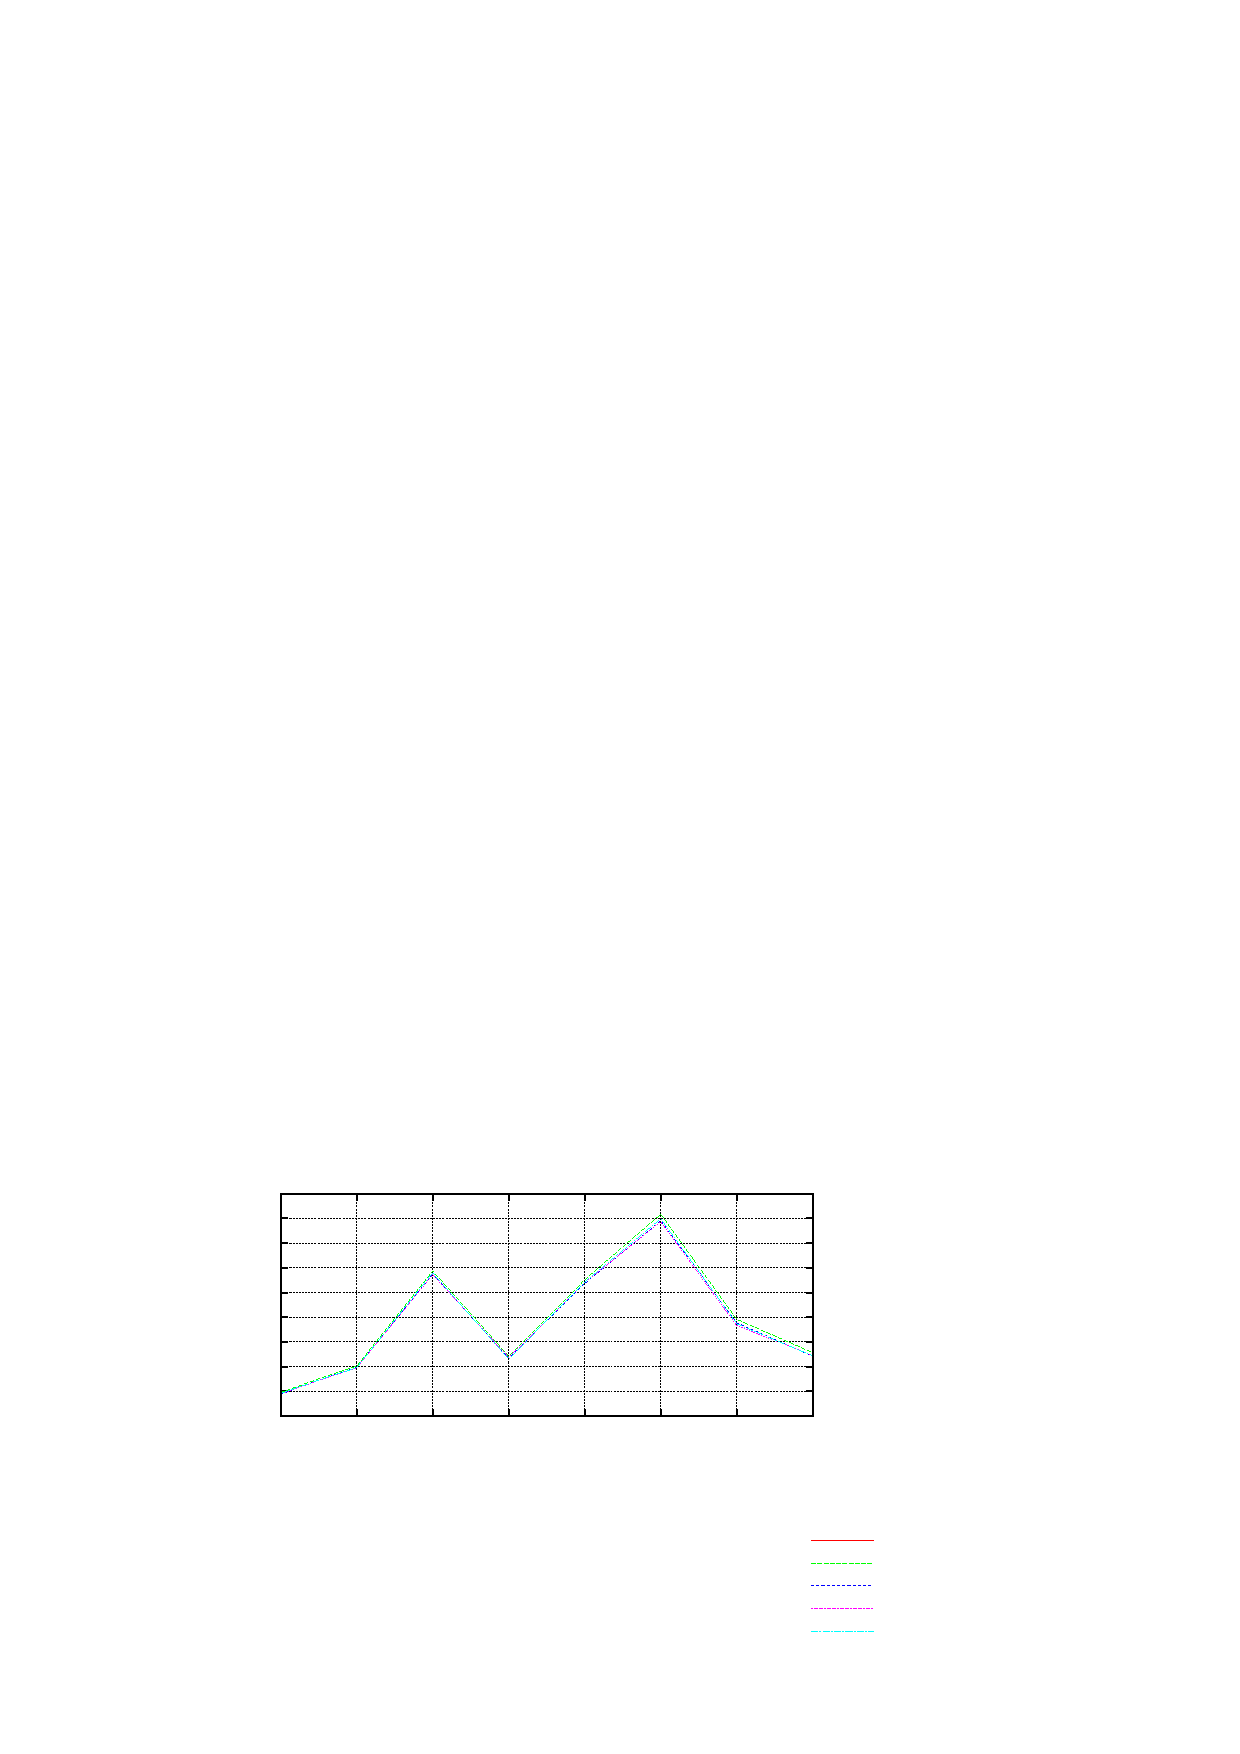
\includegraphics{ej4_frontera_connected_dense}}%
    \gplfronttext
  \end{picture}%
\endgroup
